\section{Robot}
To demonstrate the platform it was decided to make a vehicle with a manipulator controlled remotely over internet. In addition the robot should have sensors that send data (if available) continuously to the server and be able to send camera feed to the operator. Due to the possibility to expand this later with more complex functionality, the program was written in C++.
The following was used to make this vehicle:
\begin{itemize}
    \item Raspberry Pi
    \item Raspberry Pi Camera
    \item Dynamixel AX-12 Servomotors
    \item Dynamixel AX-S1 Integrated Sensor
    \item USB2Dynamixel
    \item Dynamixel SDK
\end{itemize}
\vspace{\secspace}

\textbf{Rasppberry Pi} (Pi) is a single board credit-card-sized computer. It runs on an 700 MHz ARM processor.
It has two USB inputs, ethernet, HDMI and gpio (general purpose input output) headers. 
This makes it the perfect prototyping computer for this kind of project. 
The Pi is running its operating system from a SD card, and the OS is RaspBian which is a debian based linux distro.

\begin{figure}[H]
    \centering
    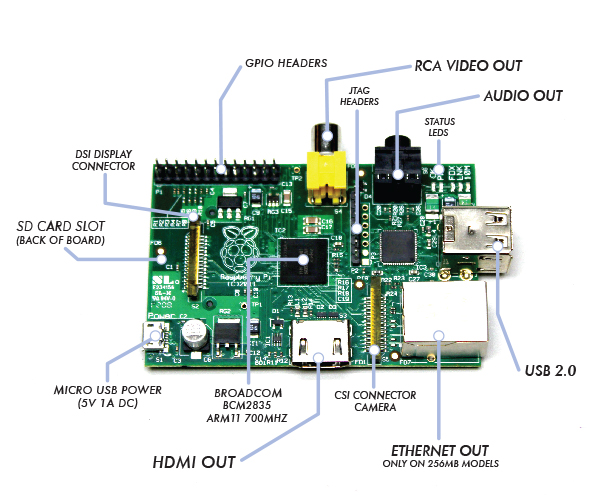
\includegraphics[width=0.7\textwidth]{graphics/Raspberry_Pi.png}	
    \caption{Raspberry Pi overview over peripherals}
    \label{fig:RPi}
\end{figure}

To control the Pi you can hook up a keyboard and a monitor directly to the board, or you can control it from another computer. 
This is achieved by using a SSH server on the Pi and a SSH client on the computer. 
SSH (Secure SHell) is a protocol that allows one computer to remotely controll another via command line. A widely known program for doing this is PuTTY. To login over SSH, you need to know the IP-address of the host. This can be done by setting the IP-address static or to scan the network to find out which IP the Pi would have. Since both of these approaches are difficult on a big network like NTNU, we had to find another approach. The solution was to connect the Pi directly to the computer via an ethernet cable. To do this we had to do some modifications, the full tutorial on how to do this see \footnote{\url{http://pihw.wordpress.com/guides/direct-network-connection/}}. To get internet access we first shared the Wi-Fi connection on the computer described here \footnote{\url{http://anwaarullah.wordpress.com/2013/08/12/sharing-wifi-internet-connection-with-raspberry-pi-through-lanethernet-headless-mode/}}. Later we used a Wi-Fi usb dongle. The driver for this dongle installed automatically and all we had to do was to configure \textit{/etc/network/interfaces}, and add the following:
\begin{verbatim}
    auto wlan0
    iface wlan0 inet dhcp
    wpa-ssid "<nameOfNetwork>"
    wpa-psk "<networkPassword>"
\end{verbatim}
We had to set up a own network to do this, because the eduroam network uses different setup.
\vspace{\secspace}

\textbf{Raspberry Pi camera}

\vspace{\secspace}

\textbf{Dynamixel AX-12 servomotors}
are motors that allows for precise controll of angle and velocity. These motors are controlled over a half duplex UART, which is a byte oriented asynchronous serial communication protocol. You can control the motors and receive feedback by sending commands to it corresponding to the control table in the datasheet [PUT REFZ H3R3]. The most important features is the control of position and velocity. The servos can work like normal servos where you can put in the desired position, and a controller inside the servo will make the servo go to that position. This position is limited to between 0-300 degrees (see datasheet). The servo can also work in so called "Endless Turn" mode, where the servos can spin infinite. Here you can only control the velocity which the motors run. "Endless Turn" mode is activated by setting the angle limits (CW Angle Limit and CCW Angle Limit) to zero.
\vspace{\secspace}

\textbf{Dynamixel AX-S1 Integrated Sensor}
is a sensor device capable of measuring sound, brightness, heat and distance to objects. It is also capable of making sound. The communication is the same as the servomotors and the sensor is connected to the same bus. 
\vspace{\secspace}

\textbf{USB2Dynamixel} \footnote{\url{http://support.robotis.com/en/product/auxdevice/interface/usb2dxl_manual.htm}} is a USB device that allows the computer to create a virtual serial port (UART) and with some other circuitry, communicate with the servos over the USB port.
This USB requires no driver installation when running linux, and since RaspBian is a linux distro this simplifies things. 
The USB2Dynamixel is inserted into one of the USB ports on the Pi and the servor motors are connected to the device.

Since the Pi also has a hardware UART driver on two of its gpio headers, we thought about if we could communicate with the servos through these pins. 
To do this we had to make the circuitry described on page 8 in the datasheet [PUT REFZ H3R3]. 
We would also have to implement our own code for the lower part of the communication (where we used a library from the manufacturer, more on that later).
UART is also widely supported by many lower end microcontrollers which don't have the support for an OS. 
Therefore using UART would mean that the code would be even more platform independent.
\vspace{\secspace}

\textbf{Dynamixel SDK} is a programming library for controlling dynamixel servo motors. 
This library is available for Windows, Mac and Linux and easy to run on the Pi. 
Since the library is written in C it is easy to use it in this C++ project.
There is a great API reference \footnote{\url{http://support.robotis.com/en/software/dynamixelsdk.htm}} with the library.
The functions treat the lower part of the communication over USB2Dynamixel.
There are functions for initializing the communication, terminate the communication, sending byte and words (16 bit), receiving byte and words, and for ping. Ping is for checking if a device is connected.
There is also a page describing platform porting \footnote{\url{http://support.robotis.com/en/software/dynamixel_sdk/sourcestructure.htm}}


\subsection{The overall system}

nice drawing

communication (because of threads)

easy to develop further

\subsection{Wiggle It}

The first step is to make a servo motor move. 

\begin{figure}[H]
    \centering
    %sett inn figure her
    \caption{Servo motor test setup}
    \label{fig:servo} 
\end{figure}

To make the servo motor move the example-program for the motor class could be used \footnote{LOCATION TO MOTOR EXAMPLE PROGRAM}. Alternative the example-file readWrite form the dynamixel library could be used \footnote{LOCATION TO READWRITE EXAMPLE FILE}. 
For this to work there are some important parameters which should be known:
\begin{itemize}
     \item ID - Each motor has its own ID. This way its possible to control which motor that should get the command. The ID need to be change in the code to the ID of the motor. If the motor ID is unknown, you could use the \textit{pingAll()} function. This will search for IDs on the bus, and print out those that are active
     \item Port - Which port the USB2Dynamixel is connected to. This is used to set up the communication to the motors. USB devices under linux can be found under \textit{/dev/usb}. When testing we used deviceIndex = 0 (\textit{/dev/usb0}).
     \item Baudnumber - used to set the speed of the bus. This should always be one, which is 1Mbit/s, unless lower speeds are needed.
\end{itemize}
\vspace{\secspace}

By replacing these parameters in the example file the servos should move back and forth when enter is pressed.


\subsection{Driving}
The next step is to make four wheels cooperate!

endless turn

setting speed

turning 

\subsection{Manipulator}

inverse kinematic (drawing)

gripper

\subsection{Testing it all with a local interface}

mouse and keyboard input

x11/xming

\subsection{Sensor}

make sound

read ir

\subsection{Exception handling}

failsafe mode

ping

threads

tried some wheels

\subsection{Future problems/challenges}
What happens if some of the wheels is disconnected? 
The answer for this question will not be covered in this report because of the timeframe, but it is an important issue that has to be resolved. 
The optimal solution is to find an algorithm that calculates the speed that the remaining wheels, so that the vehicle can obtain normal function even in failsafe mode. 
This will most likely depend on the surface under the vehicle. 


%%% Local Variables: 
%%% mode: latex
%%% TeX-master: "../report"
%%% End: 
